\section*{Einleitung}
Diese Arbeit beschäftigt sich mit der Layout-Segmentierung von Digtalisierten Dokumenten mittels Neuronaler Netzwerke.

\cref{chap:documents} beschreibt die Motivation für die Dokumentensegmetierung und aktuelle Entwicklungen im
Bereich der Dokumenten-Digitaliserung.

\cref{chap:reproduktion} nähert sich dem aktuellen Forschungsstand mittels der Reproduktion von drei Forschungsergebnissen.

\cref{chap:selfsupervised} erläuter die Methode des selbstüberwachten Lernen. Die Methode wird auf die reproduzierten Forschungen angewendet.

\chapter{Digtalisierten Dokumente}
\label{chap:documents}
% Warum scannt man Dokumente

% Was für Dokumente werden gescannt

% 
Schon in den 50er Jahren begann die Forschung im Bereich der Optischen Zeichenerkennung 
(engl. OCR)\autocite{doermann_evolution_2014}. OCR fand zuerst Anwendung in genau 
spezifizierten Problembereichen zum Beispiel die Erkennung von Druckbuchstaben einer Schreibmaschine. 
Je mehr Dokumente digitalisiert wurden, desto klare wurde es das Dokumente mehr als 
eine Kette von Zeichen sind. 


Information wird in Dokumenten auch über die Position der Zeichen und Skalierung von Zeichen vermittelt.

Zum anderen bestehen Dokumente auch aus Inhalten die semantische Bedeutung haben, aber nicht als
Zeichenkette codiert werden können. 
Zum Beispiel Textboxen.


\section{Schritte in der Verarbeitung von Dokumentenbildern}
Die Dokumentensegmetierung ist ein Vorverarbeitungsschritt für weitere Schritte der Dokumentenverarbeitung.
Eine typische Aufgabe ist die Erkennung des Leseflüsses.

Im Bereich der Bibliotheswissenschaften besteht ein großes Interesse an Klassifizierung von
Buchseiten zur besseren Erschließung.
\cite{mcconnaughey_labeled_2017} klassifizieren Buchseiten anhand von textbasierten Features in 4 Kategorien. 
Flow
\section{Auswahl und Beschreibung der Datensätze}
\textcite[985\psqq]{doermann_datasets_2014} listen 5 Aspekte die bei der Erstellung von Datensätzen zu beachten sind:
Auswahl der Daten
Datenbeschaffung
Ground Truth Definition
Ground Trouth Annotation
Speicherformat
Struktur und Organisation

\chapter{Reproduktion bisheriger Ergebnisse}
\label{chap:reproduktion}

\section{Umsetzung}
Automatische Differenzierung

\section{PyTorch}

\section{Dokumentensegmetierung mittels CNN}
1. Ansatz von \textcite{chen_convolutional_2017}
Superpixel segmentierung
Klassifizierung auf Superpixel statt Pixelebene.

2. Ansatz von \autocite{wick_fully_2017}

\section{SLIC Superpixel}
\cite{achanta_slic_2010}

\chapter{Selbstüberwachtes Lernen}
\label{chap:selfsupervised}

Jigsaw
\cite{noroozi_unsupervised_2016}
% \begin{figure}
%     \includegraphics[]{figures/graphs/exp.pdf} 
%     \caption{Image}
%   \end{figure}

\chapter{Umsetzung}

\section{Evaluierung}

\begin{figure}
    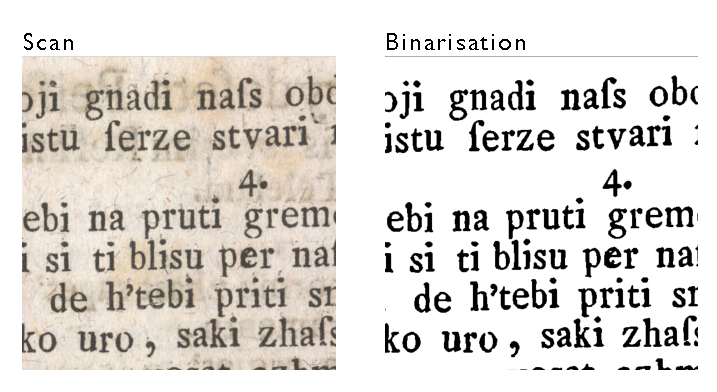
\includegraphics[]{figures/tasks/DIBCO2013-dataset.pdf} 
    \caption{DIBCO2013 Dateset Beispiel}
\end{figure}

\subsection{Metriken}
Die Evaluierung der Ergebnisse der Segmentierung erfolgt auf Pixelebene.
\cite{long_fully_2015} berechnet 4 Metriken.
Sei \(n_{ij}\) die Anzahl der Pixel der Klasse \(i\) die der Klasse \(j\) zugeordnet wurden.

% \csvautotabular{results/DIVA-HisDB.csv}

\newcommand{\resulttable}[2]{
    \begin{tabular}{l|r|r|r|r|r}%
        \hline
        \csvreader[head to column names, filter equal={\dataset}{#1}]{results/document_image_segmentation_results.csv}{}%
        {#2}
        \\\hline
        \end
        {tabular}
}

\resulttable{CB55}{\\ \name & \pixelacc & \FgPA & \meanacc & \meanIU & \fwIU}
\resulttable{CSG18}{\\  \pixelacc & \FgPA & \meanacc & \meanIU & \fwIU}
\resulttable{CSG863}{\\  \pixelacc & \FgPA & \meanacc & \meanIU & \fwIU}
